\section{Pthreads}
\begin{frame}{Pthreads implementation summary}
% Provides a set of C functions to create and manage threads and gives more control over threads than OpenMP
\begin{itemize}
  \item Pthreads: low-level threading library to create and manage threads in C
\end{itemize}

\begin{figure}
\onslide<2->{
\begin{subfigure}[t]{.4\textwidth}
    \centering
    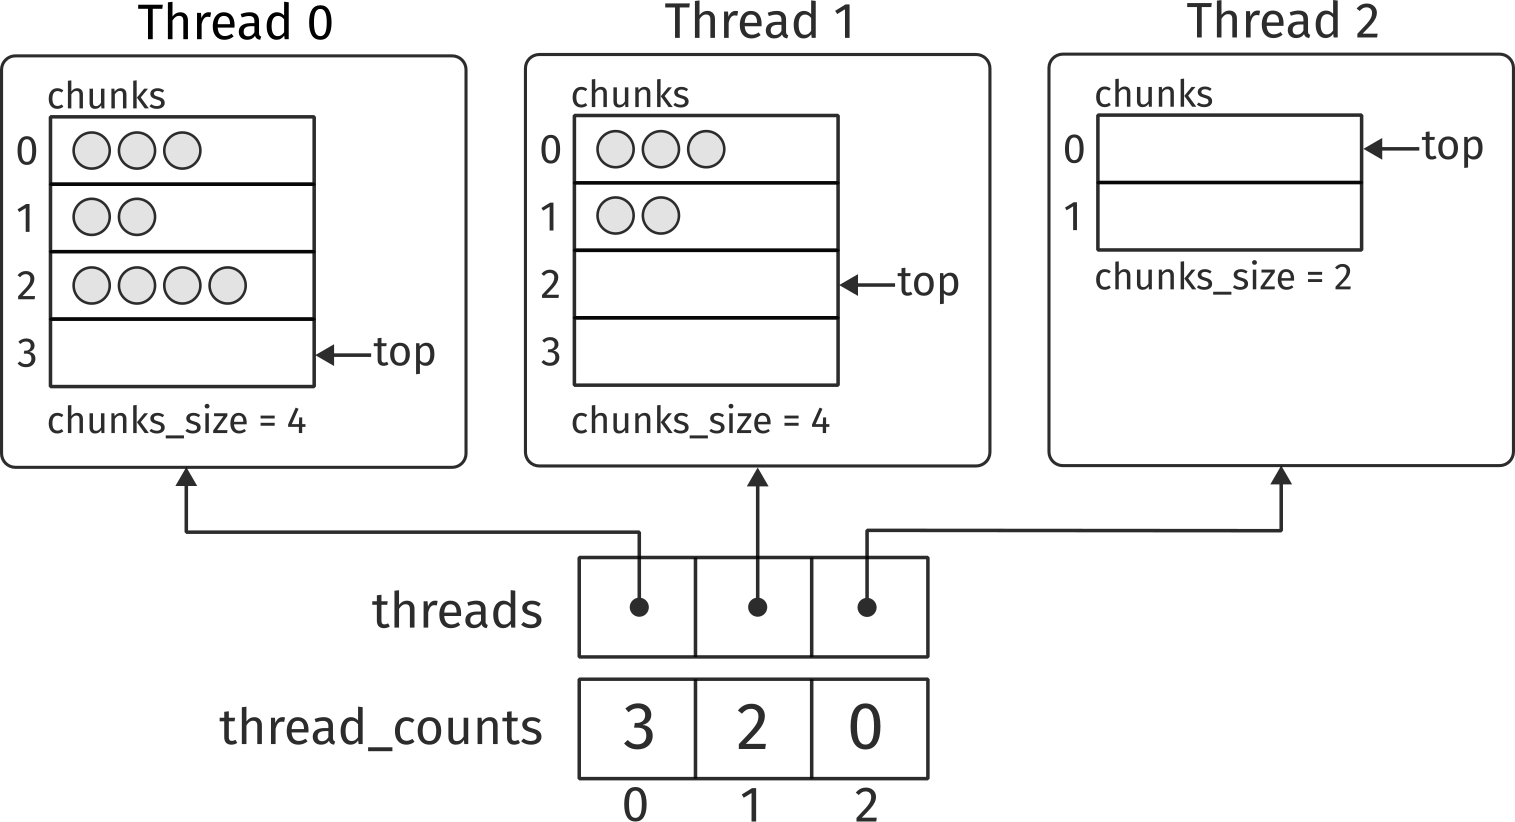
\includegraphics[width=.7\linewidth]{images/frontier_slides_3.png}
    \caption{Custom frontier data structure}
\end{subfigure}
}
\quad
\onslide<3->{
\begin{subfigure}[t]{.4\textwidth}
    \centering
    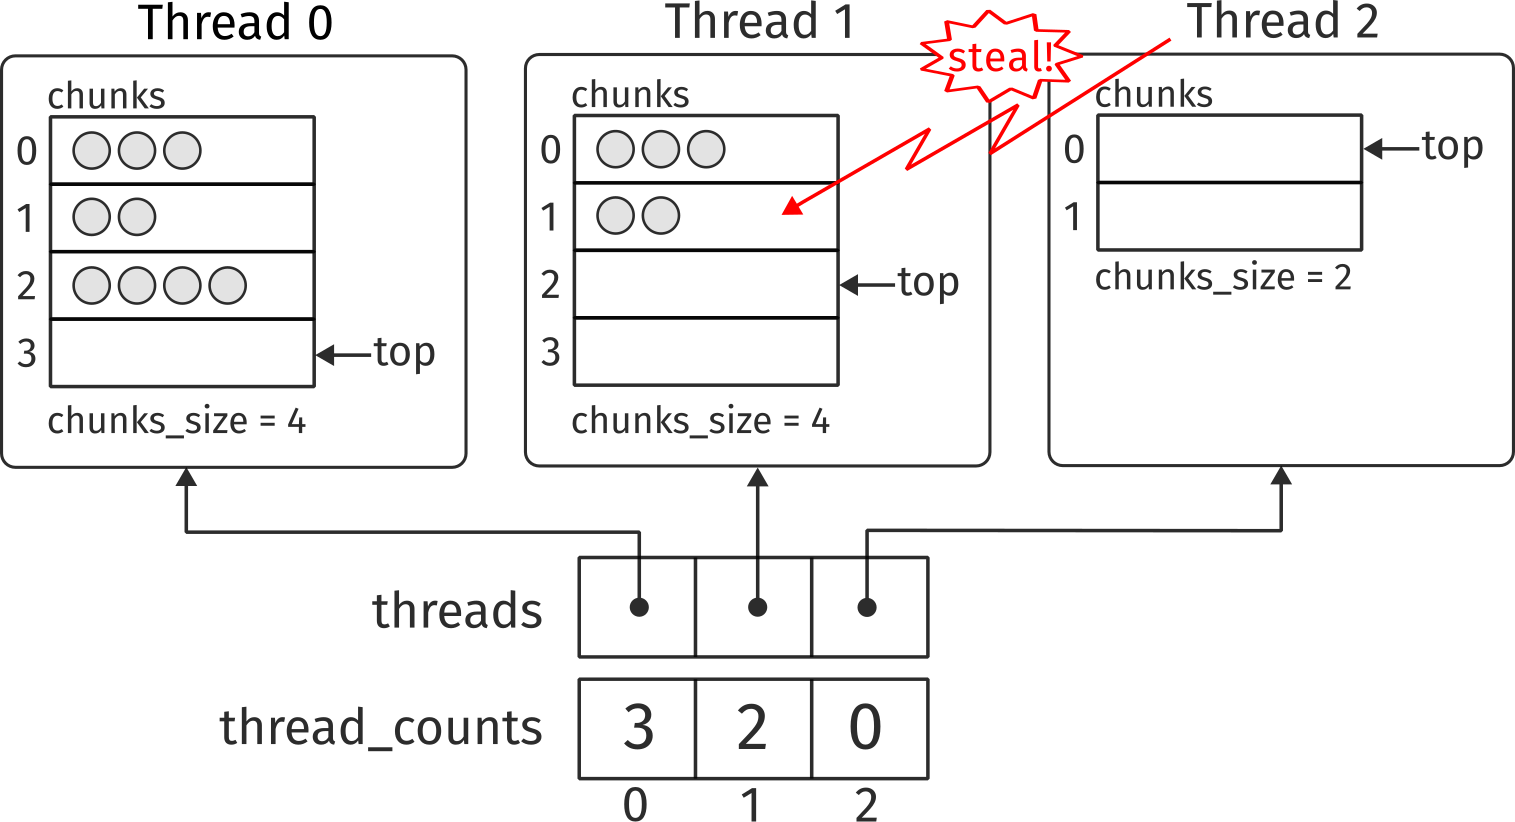
\includegraphics[width=.7\linewidth, trim={5cm 4cm 0.5cm 0}, clip]{images/frontier_slides_4.png}
    \caption{Work-stealing mechanism}
\end{subfigure}
}
\medskip

\onslide<4->{
\begin{subfigure}[t]{.4\textwidth}
    \centering
    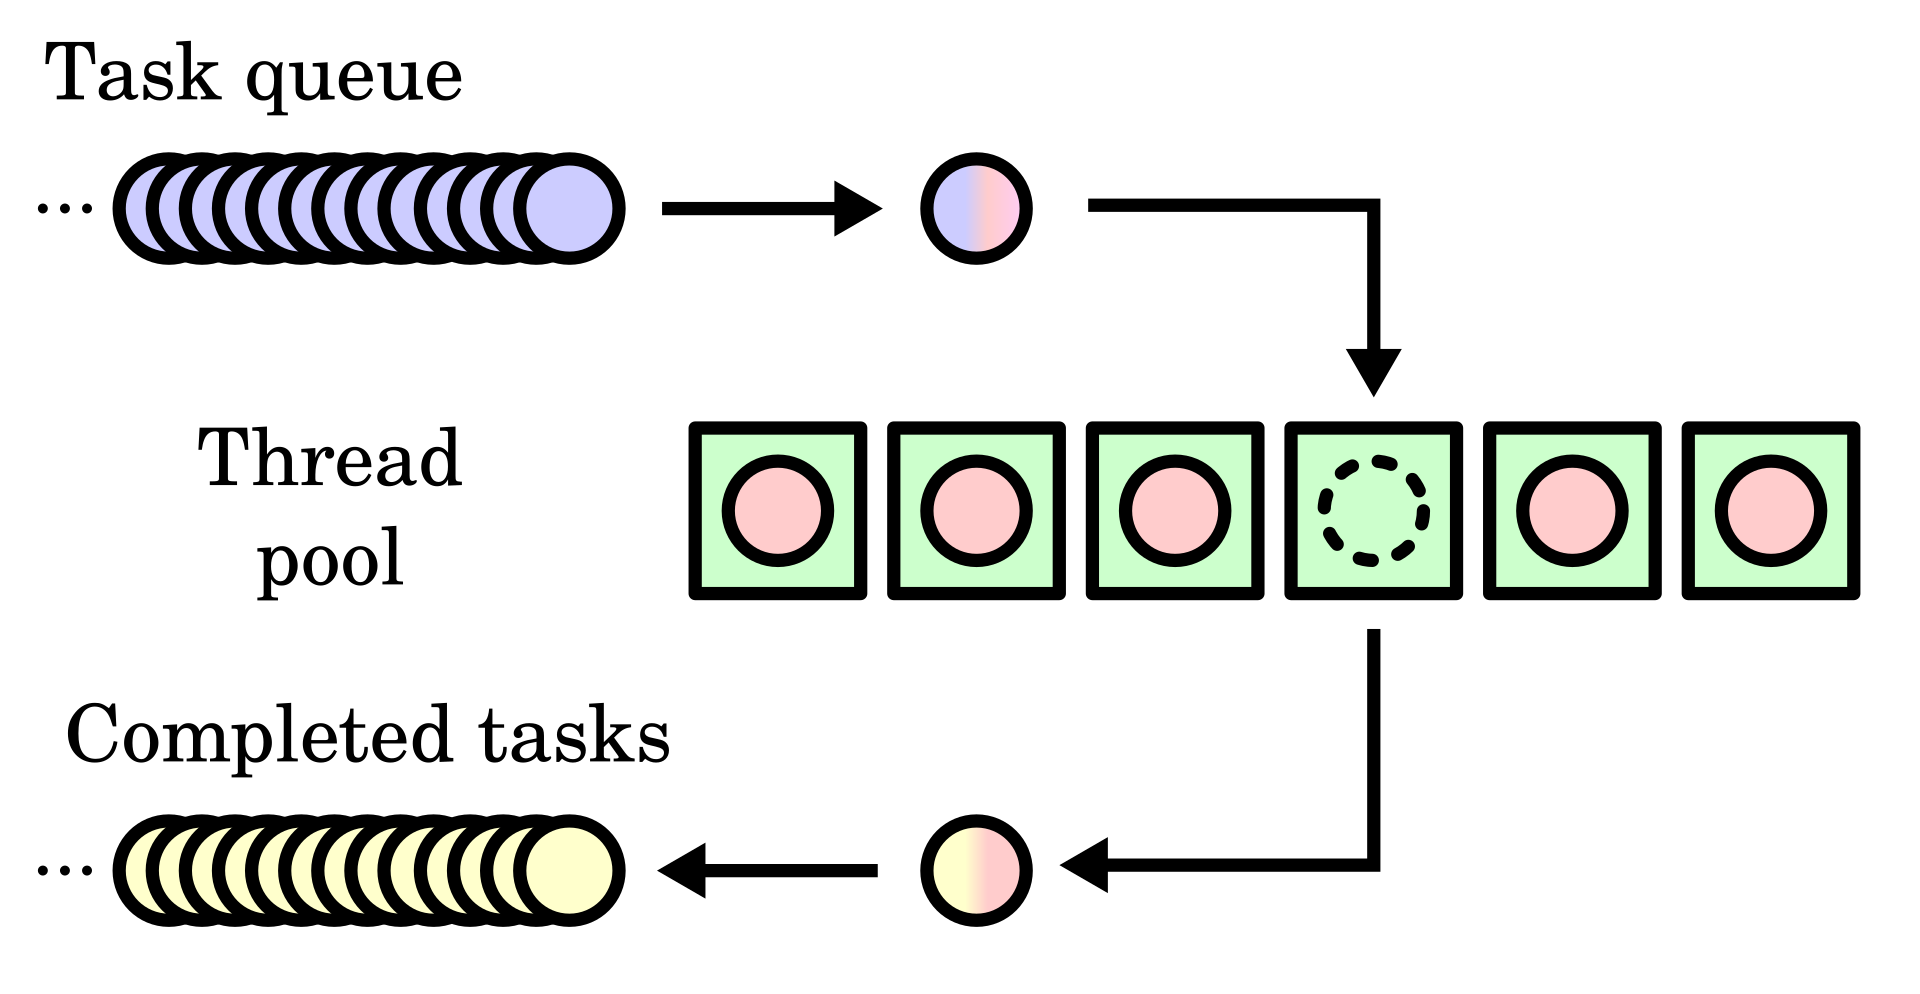
\includegraphics[width=.7\linewidth]{images/Thread_pool.png}
    \caption{Thread pool}
\end{subfigure}
}
\quad
\onslide<5->{
\begin{subfigure}[t]{.4\textwidth}
\centering
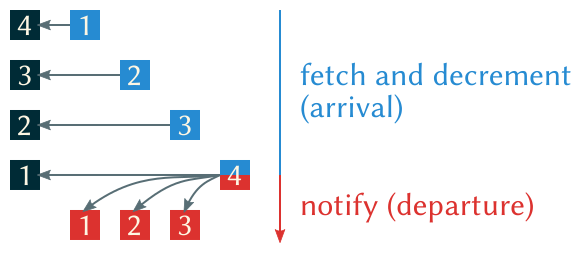
\includegraphics[width=.7\linewidth]{images/barrier.png}
\caption{Custom barrier}
\end{subfigure}
}
\end{figure}
\end{frame}

\begin{frame}{Frontier implementation}
\only<1>{
\begin{figure}
  \centering
  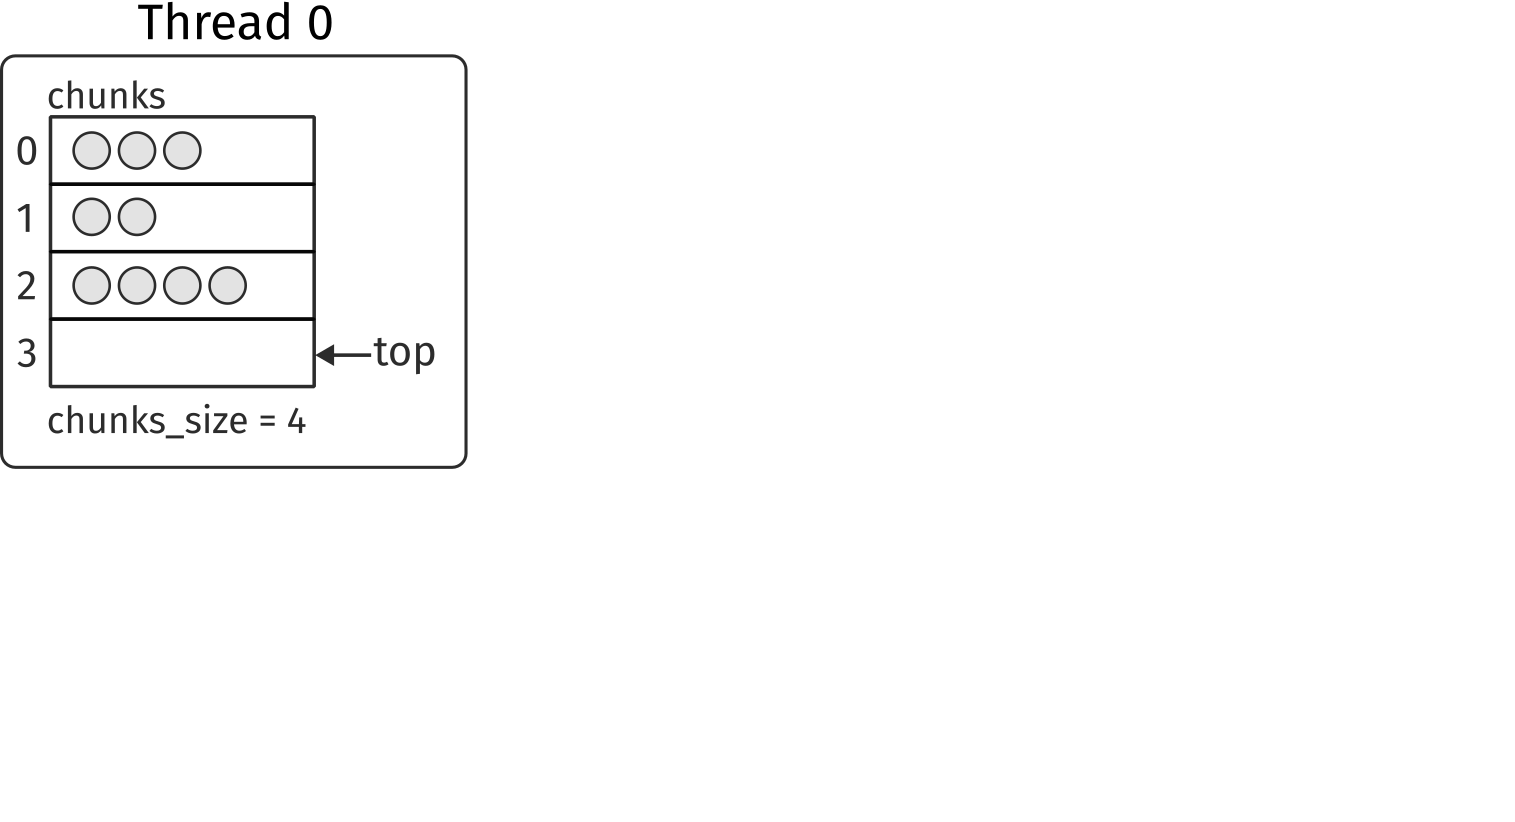
\includegraphics[width=0.8\linewidth]{images/frontier_slides_0.png}
\end{figure}
}
\only<2>{
\begin{figure}
  \centering
  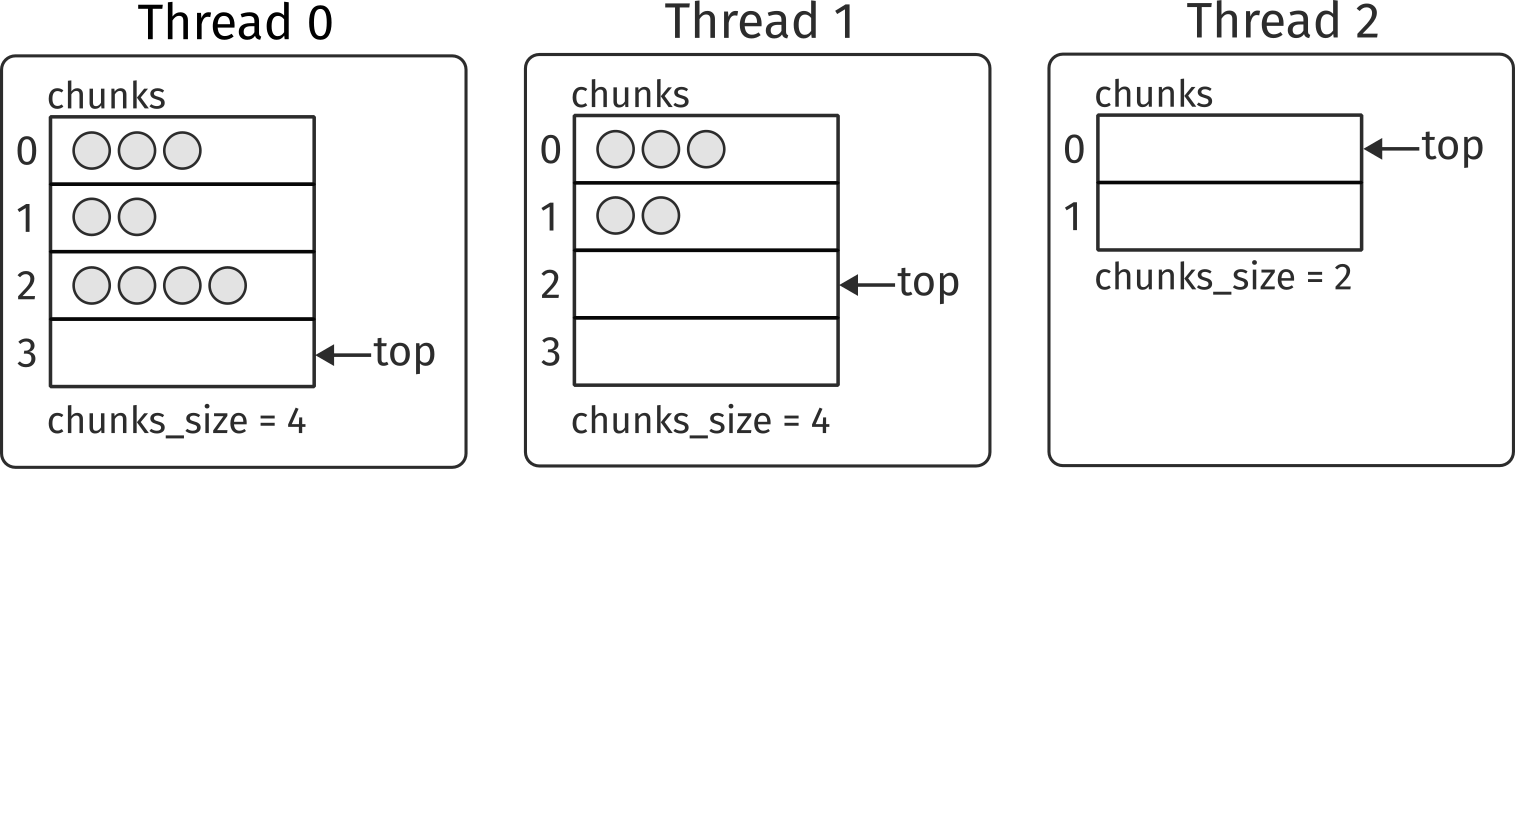
\includegraphics[width=0.8\linewidth]{images/frontier_slides_1.png}
\end{figure}
}
\only<3>{
\begin{figure}
  \centering
  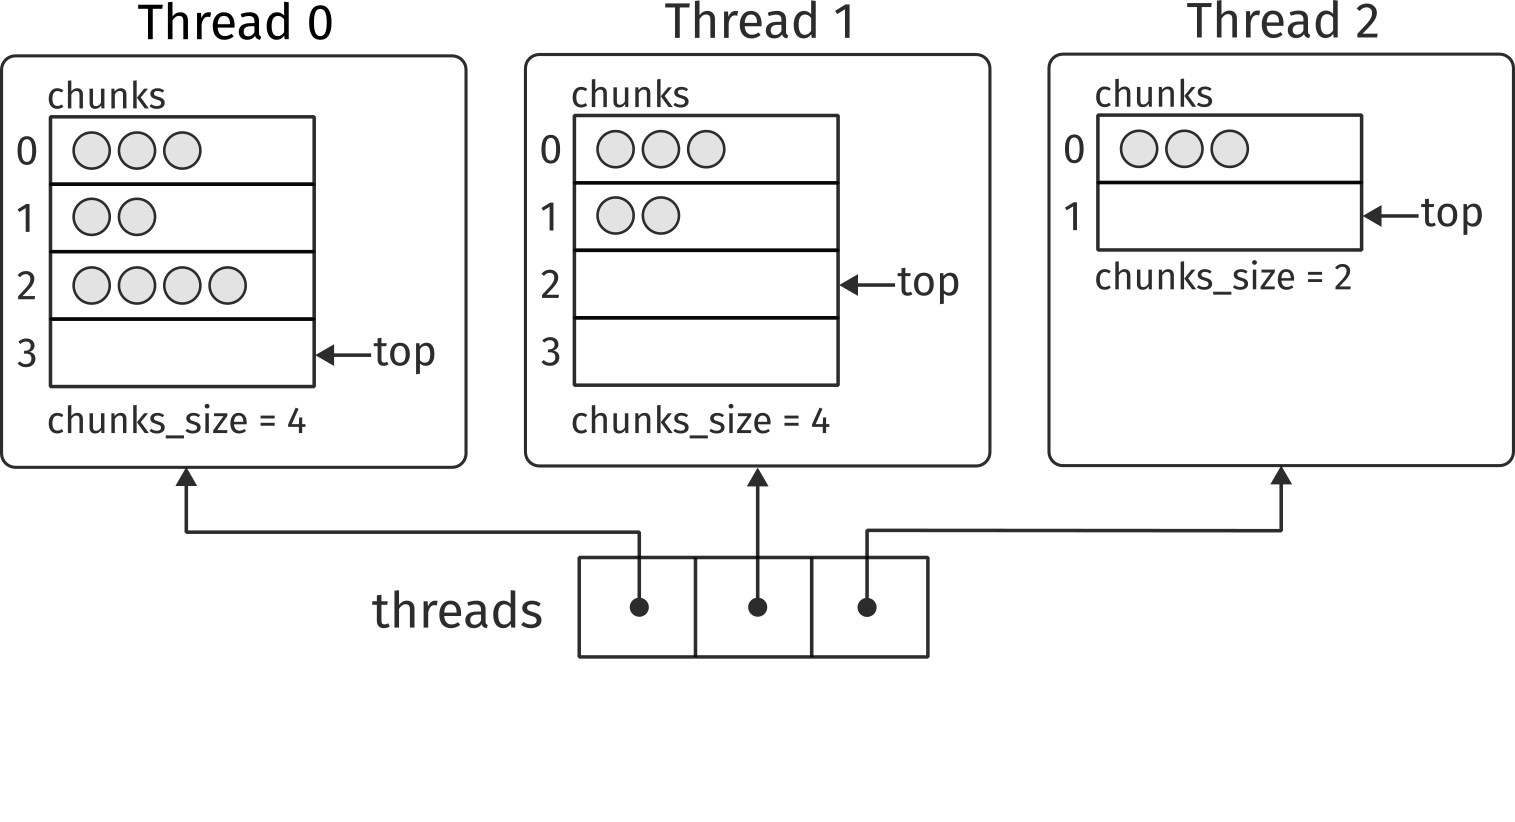
\includegraphics[width=0.8\linewidth]{images/frontier_slides_2.png}
\end{figure}
}
\only<4>{
\begin{figure}
  \centering
  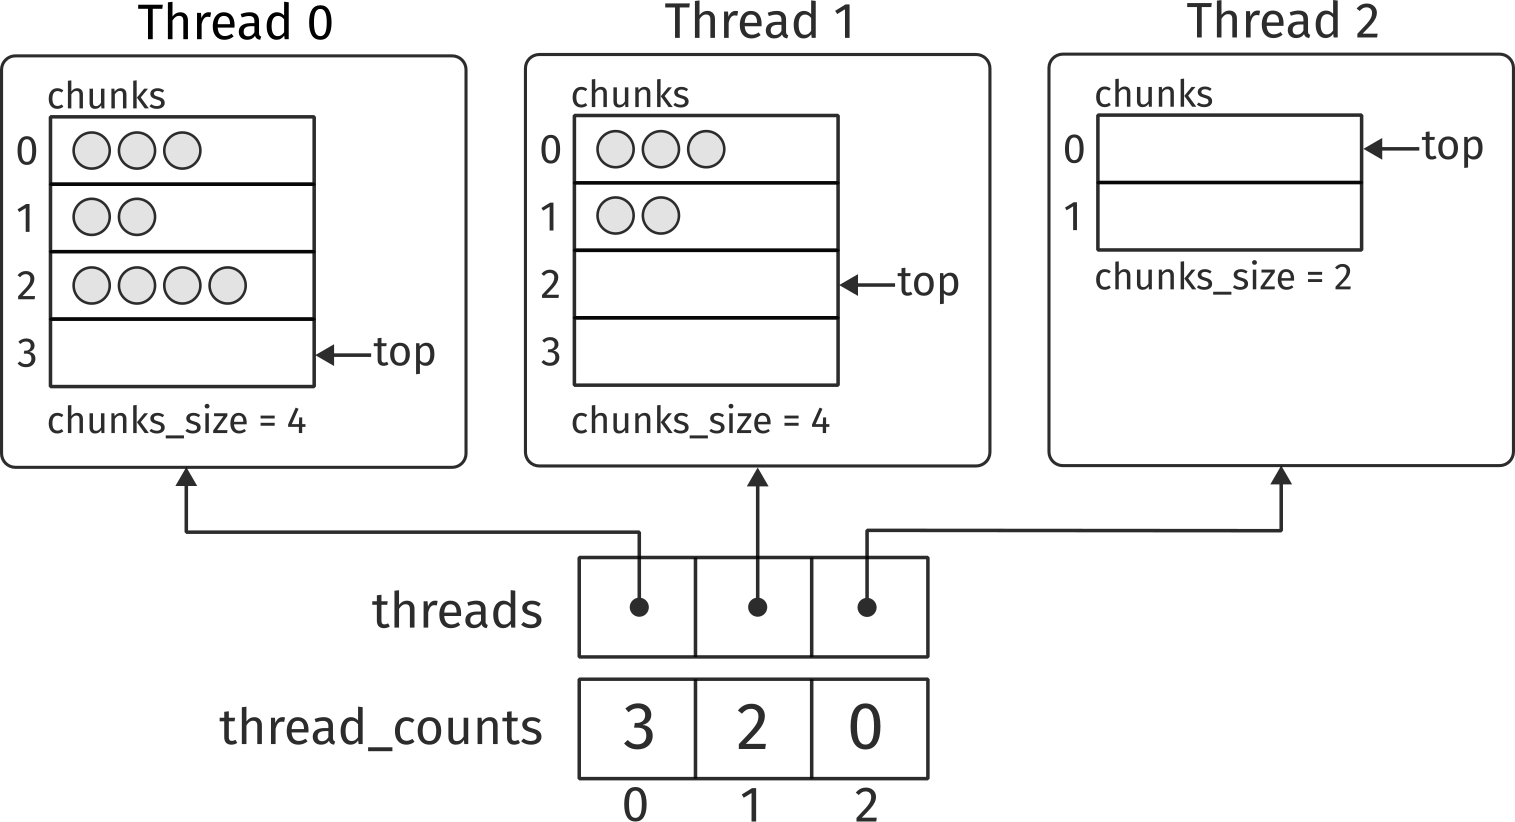
\includegraphics[width=0.8\linewidth]{images/frontier_slides_3.png}
\end{figure}
}
\end{frame}
\begin{frame}{Work-stealing mechanism}
\only<1>{
Thread 2 is out of work! It will attempt a steal soon...
\begin{figure}
  \centering
  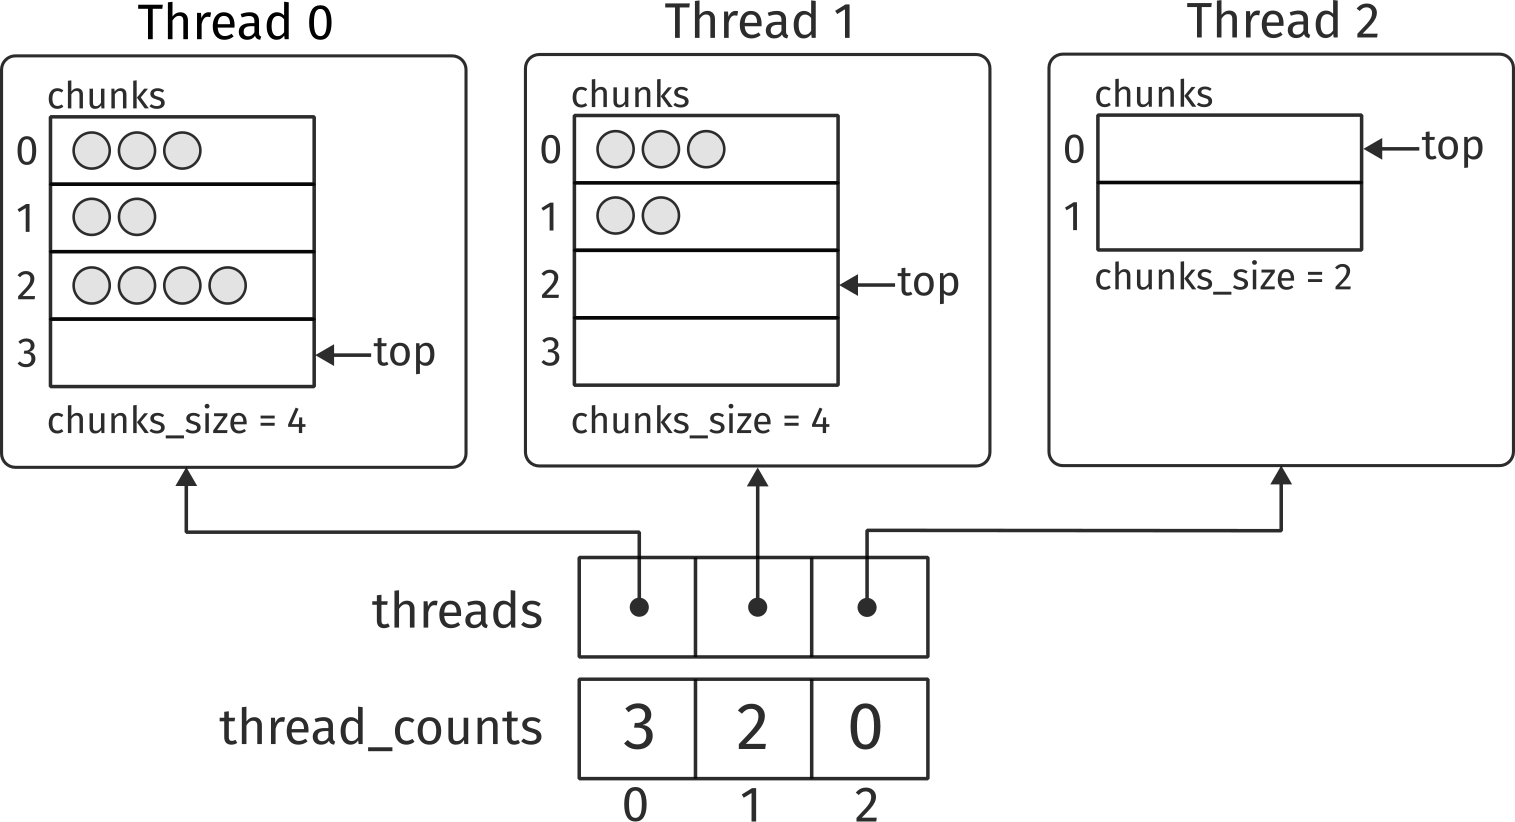
\includegraphics[width=0.8\linewidth]{images/frontier_slides_3.png}
\end{figure}
}
\only<2>{
Thread 2 steals a chunk of work from Thread 1...
\begin{figure}
  \centering
  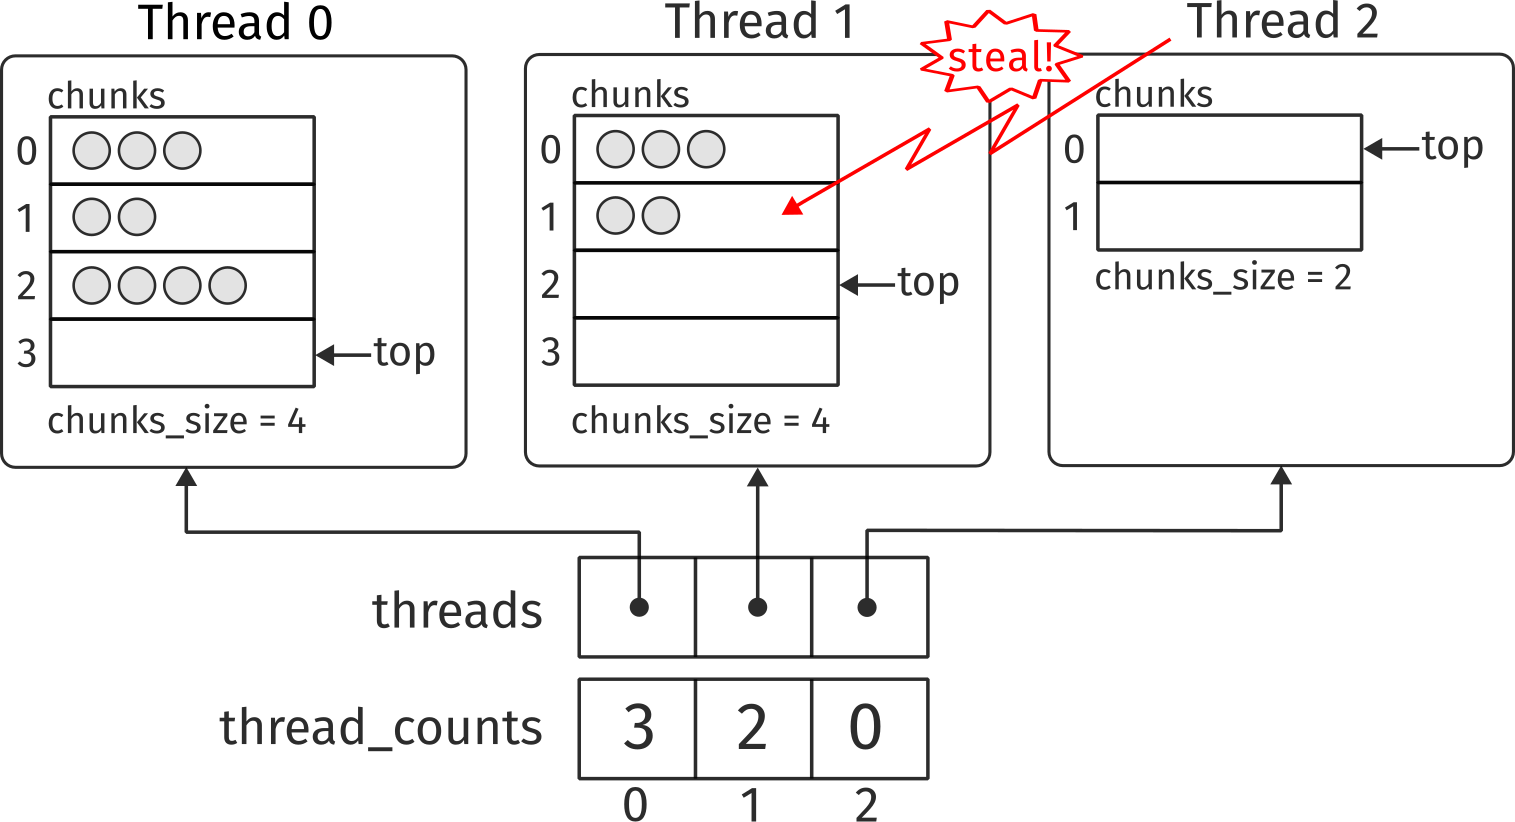
\includegraphics[width=0.8\linewidth]{images/frontier_slides_4.png}
\end{figure}
}
\only<3>{
Thread 2 processes the stolen vertices and updates the global count.
\begin{figure}
  \centering
  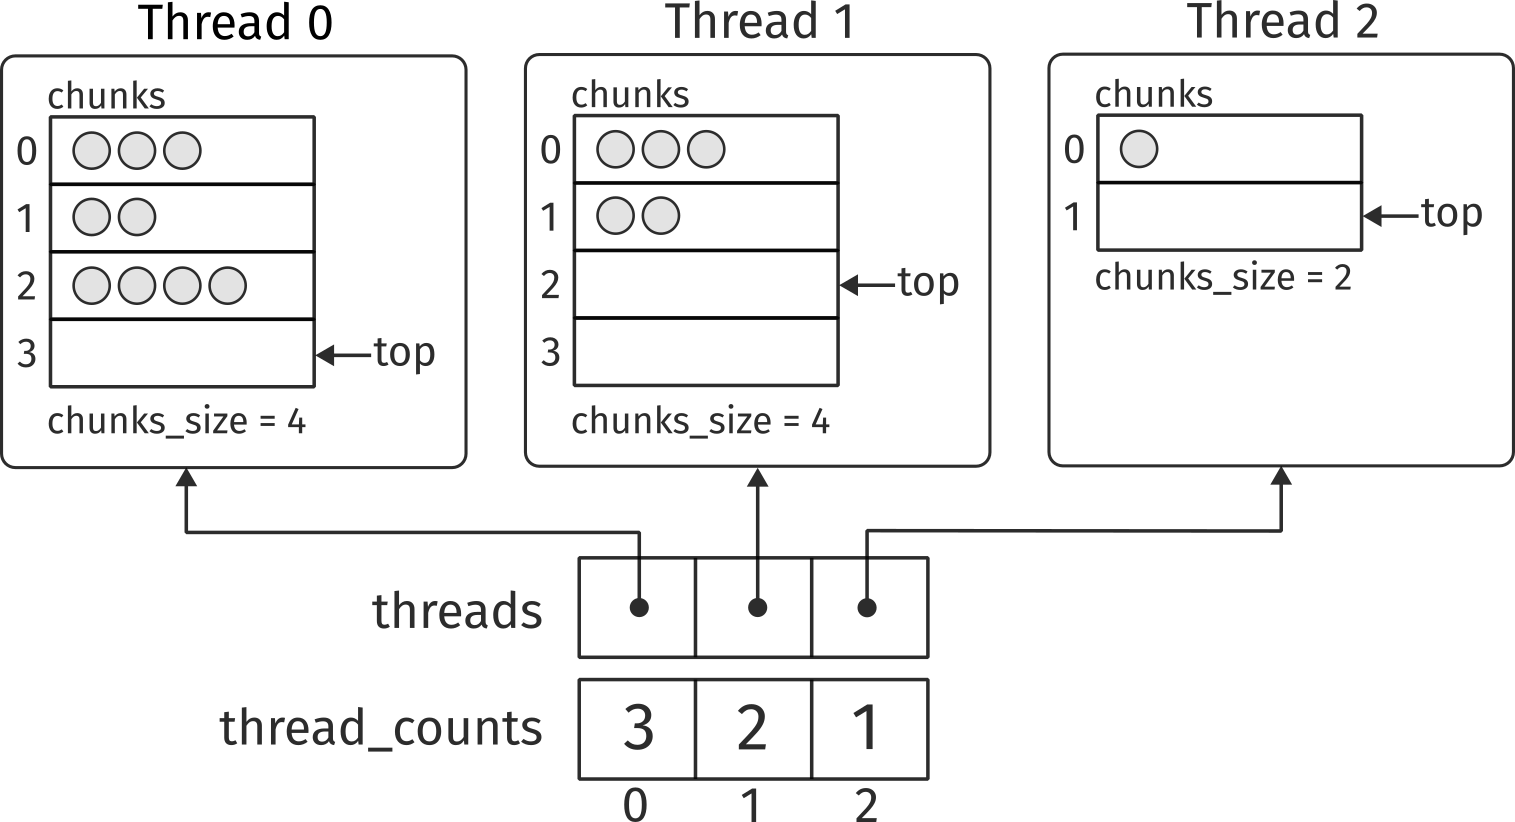
\includegraphics[width=0.8\linewidth]{images/frontier_slides_5.png}
\end{figure}
\begin{tikzpicture}[remember picture,overlay]
  \node[
    fill=yellow!30,         % background color
    text=black,             % text color
    rounded corners,
    draw=orange!80!black,   % border color
    thick,
    inner sep=6pt,
    anchor=south east,
    font=\small,
    align=center
  ] at ([xshift=-2.5cm,yshift=1cm]current page.south east)
  {Access to chunks is\\protected by mutexes.};
\end{tikzpicture}
}
\end{frame}
\begin{frame}{Thread pool}
\begin{itemize}
  \item Optimization to avoid repeated thread creation
  \item When the program is run, a group of threads is spawned
  \item At the beginning of each BFS run, the threads are awaken
  \begin{enumerate}
    \item Process own chunks
    \item Steal work from other threads
  \end{enumerate}
\end{itemize}
\begin{figure}
  \centering
  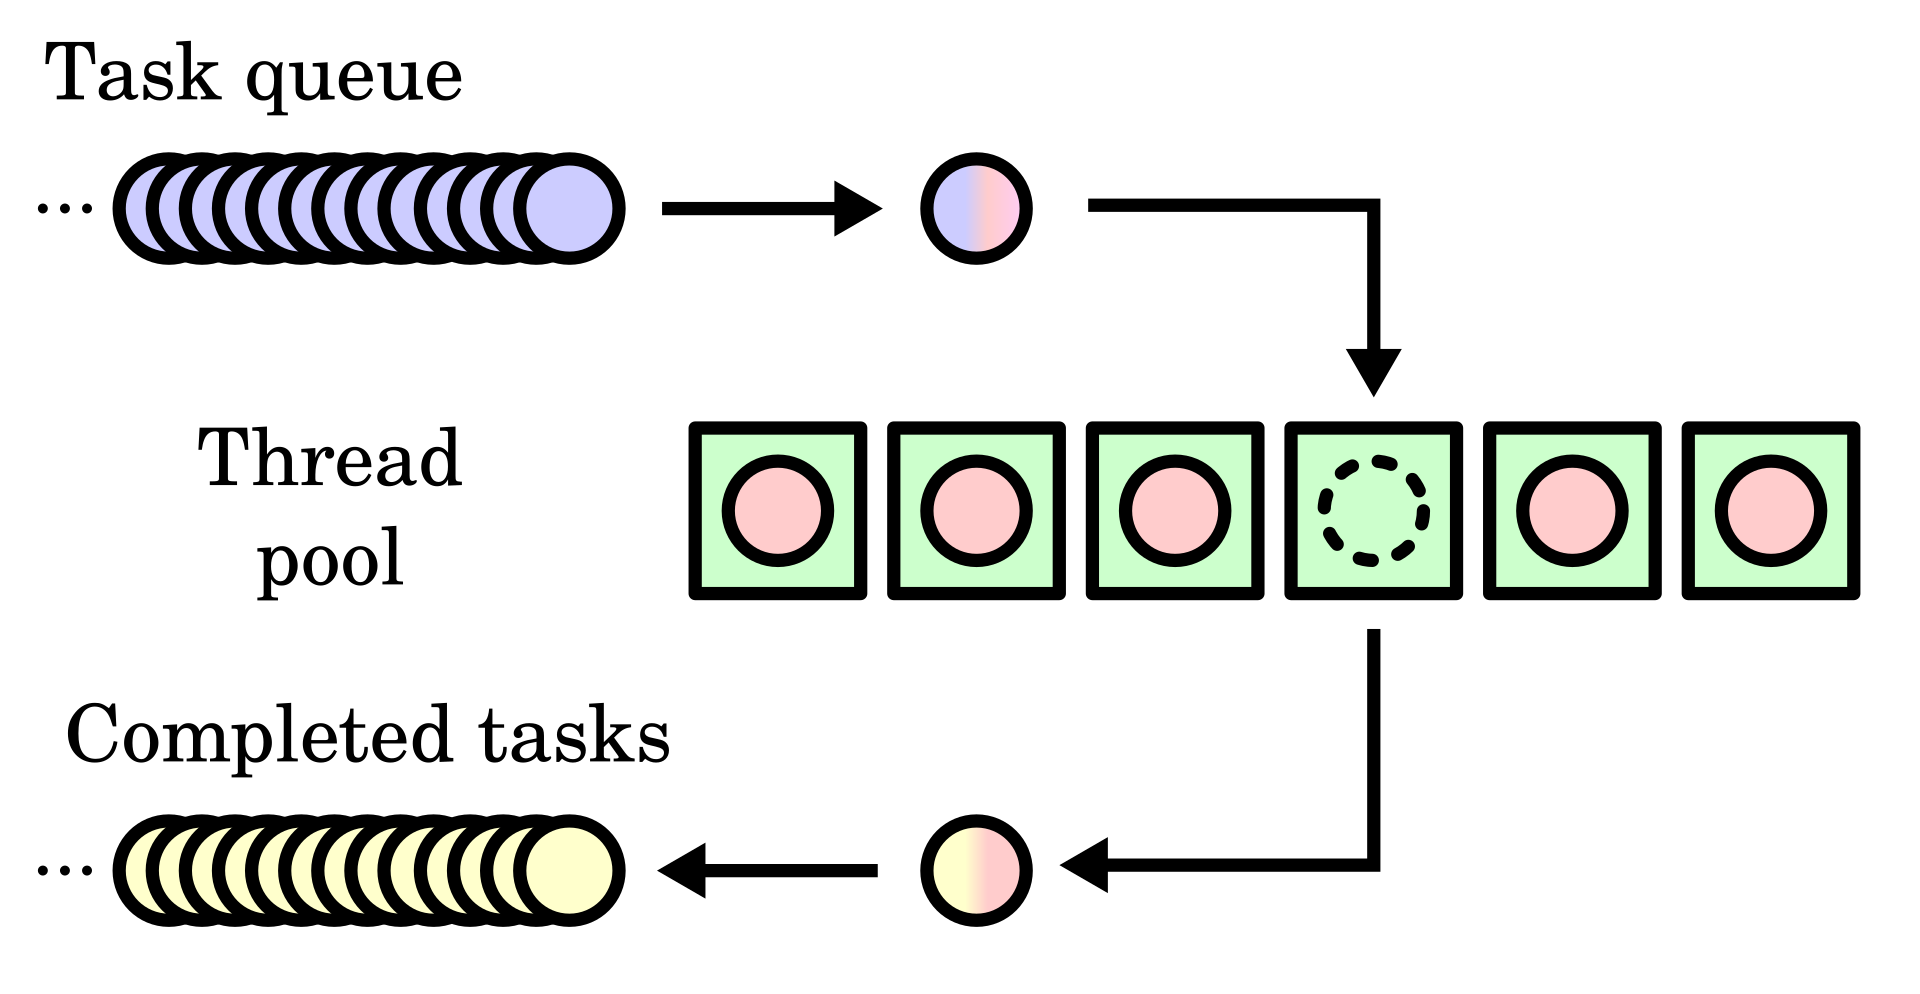
\includegraphics[width=0.5\linewidth]{images/Thread_pool.png}
\end{figure}
\end{frame}
\begin{frame}{Sense-Reversal Centralized Barrier}
  \begin{columns}[c] % split into two columns
    % Left column: bullets
    \begin{column}{0.5\textwidth}
      \begin{itemize}
        \item Barrier: point that threads must reach before any can proceed
        \item Procedure:
        \begin{enumerate}
          \item Threads decrease global counter and wait
          \item Last thread resets counter + increments distance
          \item All threads are released together
        \end{enumerate}
      \end{itemize}
    \end{column}

    % Right column: diagram
    \begin{column}{0.5\textwidth}
      \begin{figure}
        \centering
        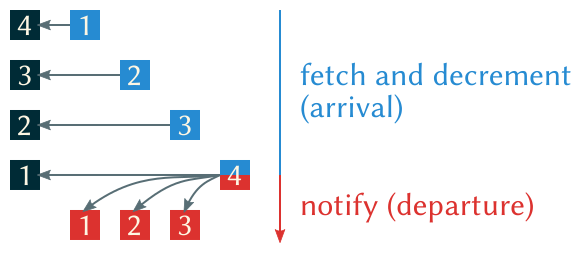
\includegraphics[width=\linewidth]{images/barrier.png}
      \end{figure}
    \end{column}
  \end{columns}
\end{frame}